\documentclass[a4paper]{article}

%% Language and font encodings
\usepackage[english]{babel}
\usepackage[utf8x]{inputenc}
\usepackage[T1]{fontenc}

%% Sets page size and margins
\usepackage[a4paper,top=3cm,bottom=2cm,left=3cm,right=3cm,marginparwidth=1.75cm]{geometry}

%% Useful packages
\usepackage{amsmath}
\usepackage{graphicx}
\usepackage[colorinlistoftodos]{todonotes}
\usepackage[colorlinks=true, allcolors=blue]{hyperref}

\title{Comparison of turbulence models}
\author{Aleksander Kufel}

\begin{document}
\maketitle

\begin{abstract}
This is a report on the differenece between Reynolds-Averaged Stress modelling and Large Eddy Simulation modelling. The conclusions are made based on simulations performed in OpeanFoam.
\end{abstract}

\section{Introduction}

To conclude the difference between RAS and LES turbulence models I performed two simulations in OpenFoam. Both have the same initial conditions and geometry. The mesh has been created with blockMesh. The flow is modeled as 2-dimensional. PisoFoam solver has been used to perform the calculations. It is a transient solver for incompressible, turbulent flow, using the PISO algorithm. To assure that the flow is turbulent, inlet velocity was calculated with the assumption of Reynolds number. 

\section{Theory}

\subsection{Reynolds-Averaged Stress modelling}
Reynolds-Averaged Stress (RAS) model is the most complete classical turbulence model. In these models, the eddy-viscosity hypothesis is avoided and the individual components of the Reynolds stress tensor are directly computed. These models use the exact Reynolds stress transport equation for their formulation. They account for the directional effects of the Reynolds stresses and the complex interactions in turbulent flows. Reynolds stress models offer significantly better accuracy than eddy-viscosity based turbulence models, while being computationally cheaper than Direct Numerical Simulations and Large Eddy Simulations.
    

\subsection{Large Eddy Simulation modelling}
Large eddy simulation (LES) is a mathematical model for turbulence used in computational fluid dynamics. It was initially proposed in 1963 by Joseph Smagorinsky to simulate atmospheric air currents, and first explored by Deardorff. LES is currently applied in a wide variety of engineering applications, including combustion, acoustics, and simulations of the atmospheric boundary layer.

The simulation of turbulent flows by numerically solving the Navier–Stokes equations requires resolving a very wide range of time and length scales, all of which affect the flow field. Such a resolution can be achieved with direct numerical simulation (DNS), but DNS is computationally expensive, and its cost prohibits simulation of practical engineering systems with complex geometry or flow configurations, such as turbulent jets, pumps, vehicles, and landing gear.

The principal idea behind LES is to reduce the computational cost by ignoring the smallest length scales, which are the most computationally expensive to resolve, via low-pass filtering of the Navier–Stokes equations. Such a low-pass filtering, which can be viewed as a time- and spatial-averaging, effectively removes small-scale information from the numerical solution. This information is not irrelevant, however, and its effect on the flow field must be modeled, a task which is an active area of research for problems in which small-scales can play an important role, such as near-wall flows , reacting flows, and multiphase flows.
\section{Geometry}

The geometry was implemented in blockMeshDict file and the mesh was created with blockMesh. Here is the view of the geometry opened in ParaView with added dimensions:
\begin{figure}[h!]
\centering
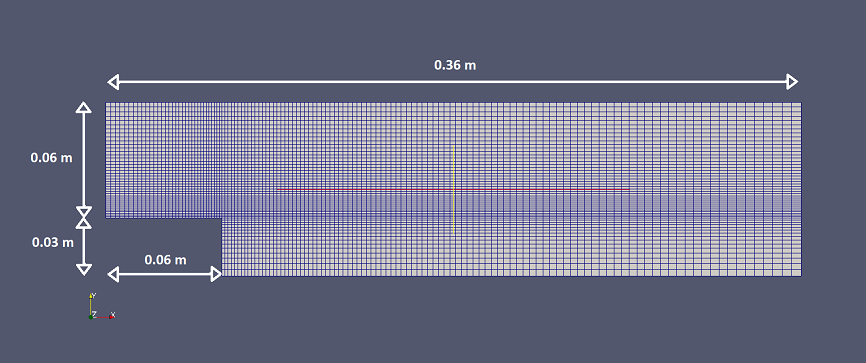
\includegraphics[scale=0.7]{geometry}
\caption{View of the geometry opened in ParaView with added dimensions}
\label{fig:geometry}
\end{figure}

\section{Simulation}
The cases were set up based on PitzDaily case from tutorial cases. The case was adopted to the geometry. The geometry I used was created by József Nagy and it is available \href{https://github.com/jnmlujnmlu/OpenFOAMTeaching/tree/master/JozsefNagy}{here}.

\subsection{Initial conditions}
As said before, to assure that the flow is turbulent, inlet velocity was calculated with the assumption of Reynolds number. I set the Reynolds number value to 50000. The calculation of inlet velocity is shown underneath. There are also two initial inlet values that need to be calculated for RAS model simulation as I use k-$\varepsilon$ model: turbulent kinematic energy (k) and turbulence dissipation rate ($\varepsilon$).

\[U = \frac{Re * nu}{L} = \frac{50000 * 10^{-5}}{0.06}=8.333\]
\[k = 1.5*(U*T_i)^2= 1.5*(8.333*0.05)^2=0.260\]
\[\varepsilon = \frac{0.09^{\frac{3}{4}}*k^{\frac{3}{2}}}{0.07*L}= \frac{0.09^{\frac{3}{4}}*0.26^{\frac{3}{2}}}{0.07*0.06}=5.199\]
\subsection{Turbulence model}
The turbulence model was set in the turbulenceProperties file in constant folder. 

\subsection{Results}
Here are results of both simulations. These figures below show velocity field for x direction in the simulated flows at time steps: 0.05, 0.1, 0.15 and 0.2 seconds after the start.\newpage

\begin{figure}[h!]
\centering
\includegraphics[scale=0.6]{RAS_Model}
\caption{Velocity in the x direction for RAS simulation}
\label{fig:RAS_Model}
\end{figure}

\begin{figure}[h!]
\centering
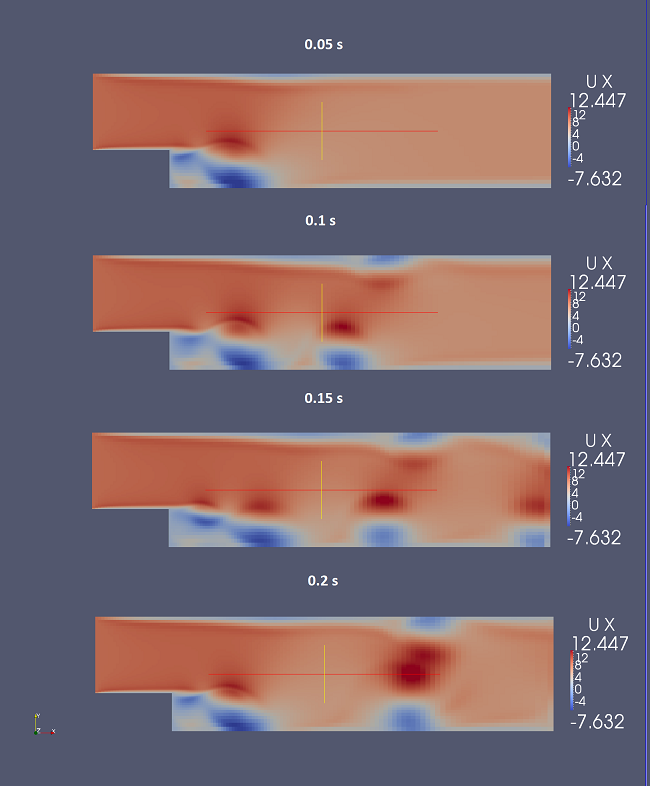
\includegraphics[scale=0.6]{LES_Model}
\caption{Velocity in the x direction for LES simulation}
\label{fig:LES_Model}
\end{figure}

\section{Conclusion}
Performed simulations shows visible differences between Reynolds-Averaged Stress and Large Eddy Simulation turbulence modelling. For the first model we can
see a region of backflow after the place where height of the flow geometry changes. In the case of Large Eddy Simulation we can also see a few vertices expanding in the flow. The conclusion of those result is compliant with the theory. The RAS model shows averaged values and can be used in cases where the details of the flow are not important. The LES model shows more details while it is still not so computably expensive.
\section{References}
\begin{enumerate}
\item \href{https://www.youtube.com/channel/UCjdgpuxuAxH9BqheyE82Vvw}{József Nagy YouTube Chanel} 
\item \href{https://en.wikipedia.org/wiki/Large_eddy_simulation}{Wikipedia - Large Eddy Simulation}
\item \href{https://www.openfoam.com/documentation/cpp-guide/html/pisoFoam_8C.html}{OpenFoam Documentation - information about the pisoFoam solver}
\item \href{https://en.wikipedia.org/wiki/Reynolds_stress_equation_model}{Wikipedia - Reynolds-Averaged Stress modelling}
\item \href{https://github.com/jnmlujnmlu/OpenFOAMTeaching/tree/master/JozsefNagy}{Github - József Nagy materials (blockMeshDict)}
\end{enumerate}

\end{document}